\documentclass[12pt]{article}
\usepackage{geometry} % see geometry.pdf on how to lay out the page. There's lots.
\usepackage{graphicx}
\geometry{a4paper} % or letter or a5paper or ... etc
% \geometry{landscape} % rotated page geometry

% See the ``Article customise'' template for come common customisations

\title{Report on Visualization Project}
\author{Daiqi Linghu, Dunzhu Li, Yiran Ma}
\date{} % delete this line to display the current date


% define argmin
\usepackage{amsmath}
\newcommand{\argmin}{\operatornamewithlimits{argmin}}
\newcommand\norm[1]{\left\lVert#1\right\rVert}

%%% BEGIN DOCUMENT
\begin{document}

\maketitle
%\tableofcontents

\section{Introduction}

\section{Algorithm}
\subsection{Optimization}
In the code (BSGD.m), we solve the following optimization problem:
\begin{equation*}
\argmin_{U,V,a,b}\frac{\lambda}{2}\left(\norm{U}^2+\norm{V}^2+\norm{a}^2+\norm{b}^2\right)+
\sum_{(i,j)\in S}\left(  Q_{i,j}  \right)^2
\end{equation*}
where $Q_{i,j}=(u_i^T v_j + a_i + b_j +\mu-Y_{i,j})$. Then,

\begin{equation*}
\frac{\partial{J}}{\partial{U_{l}}}=\lambda U_{l}+\sum_{(i,j)\in S}2Q_{i,j}1_{i=l}V_{j}
\end{equation*}


\subsection{Visualization}

\section{Implementation}
\subsection{Find U \& V} 
To solve the optimization problem with Bias-SGD, we simply divide the data by 5 fold, use 4 folds as training data and 1 fold as test data to find the optimal damping parameter $\lambda$  and number of iteration. The step size $\eta$ is chosen as 1e-2 and is decreased by 10\% for each iteration. From the results shown below (Fig. 1), we choose $\lambda=25$. For $\lambda=25$, the out-of-sample error is still decreasing at the 100th iteration (Fig. 1), however, the improvement is minimal. Therefore, we choose the number of iteration as 100.   

\begin{figure}[h!]
  \centering
      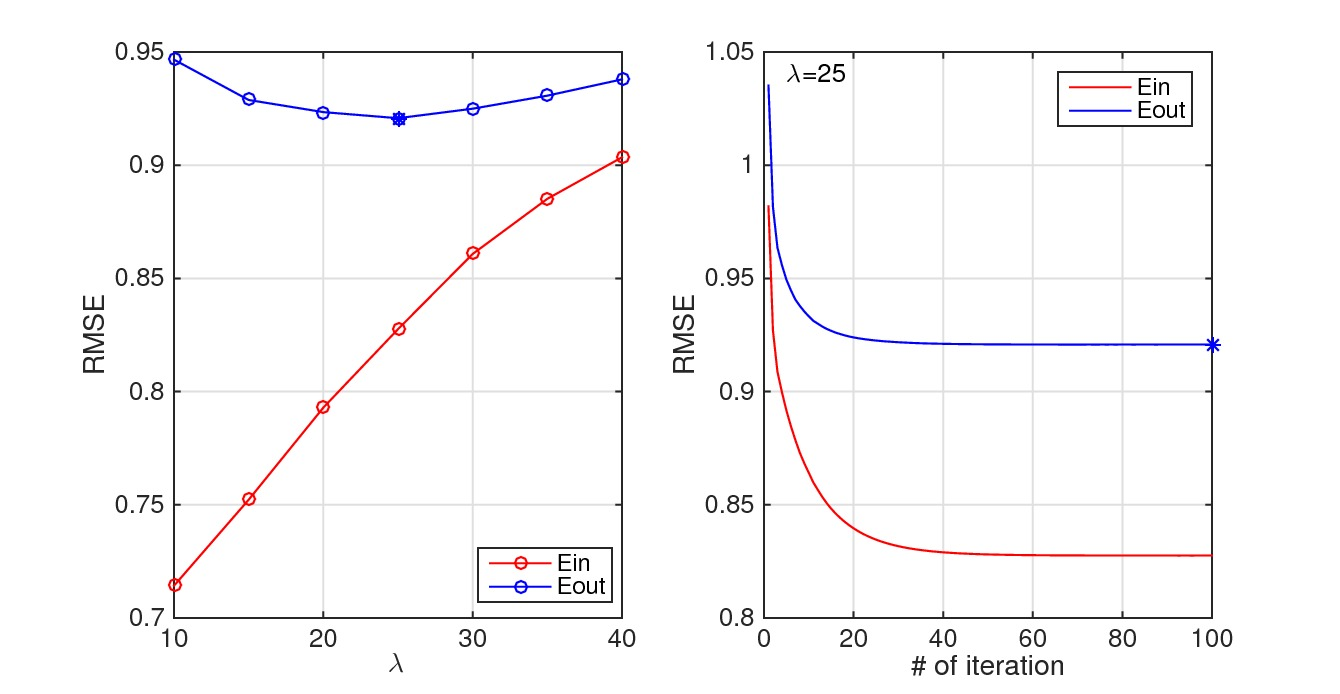
\includegraphics[width=1.0\textwidth]{testparameter}
  \caption{RMS error vs. Parameter}
\end{figure}


\subsection{Projection}



\end{document}